\documentclass[12pt]{article}
\usepackage[T1]{fontenc}
\usepackage{lmodern}
\usepackage[margin=1in]{geometry}
\usepackage[none]{hyphenat}
\usepackage{booktabs}
\usepackage{tikz}
\usetikzlibrary{positioning,arrows.meta}
\linespread{1.35}
\sloppy
\setlength{\parskip}{0.4em}

\title{Ecosystem Salience: How Platform Rules Direct Complementor Attention\\[0.8em]
\normalsize\textbf{SYNTHETIC TEST PAPER, NOT REAL RESEARCH}}
\author{Ada Marrow\\ Northfield School of Management (fictional)
\and Tobias Lenk\\ Carraway University (fictional)}
\date{}

\begin{document}
\maketitle

\begin{abstract}
\noindent Firms that build products on digital platforms, called complementors, usually serve more than one platform, and their managers cannot attend to all of them at once. We develop a conceptual account of how platform rules shape which platforms get a complementor's attention. Our core claim is that platform rules direct complementor attention through ecosystem salience and through the legitimacy that platform openness confers, and that the resulting allocation of attention decides which platforms a complementor exits. We state five propositions linking rule change frequency, rule enforcement, platform dependence, openness, and governance intensity to complementor attention, and a sixth proposition on platform exit. The account applies to complementors that serve two or more platforms whose owners set rules unilaterally. All firms and people in this paper are fictional.
\end{abstract}

\section{Introduction}

A small software firm that sells plug-ins on two design platforms faces a problem that its engineers describe in plain terms: there is never enough time to keep both versions current. Each platform revises its developer terms, its review process, and its technical interfaces on its own schedule. Every revision creates work. The firm's managers must decide, week by week, which platform gets their attention and which one waits.

This paper is about that decision. We ask how the rules that platform owners set shape the way complementors divide their managerial attention across the platforms they build for. The question matters because attention is the scarce input in small complementor firms. A complementor that neglects a platform falls behind its rules, loses visibility with users, and may eventually leave. A platform owner that understands where complementor attention goes can predict which complements will be kept current on its platform and which will decay.

Our central construct is ecosystem salience. We argue that platform rules shape which platforms get a complementor's attention through ecosystem salience. Rule change frequency, the enforcement of rule changes, and the complementor's dependence on a platform each raise that platform's ecosystem salience, and ecosystem salience in turn pulls attention toward the platform. Openness, the extent to which a platform's rules give every complementor the same published terms, is a second route: it directs attention through the legitimacy it confers on a platform. The argument ends in exit. The attention a platform loses decides whether the complementor keeps building for it, and this link from attention to exit is part of our core claim, because it is why platform owners should care where complementor attention goes. A further proposition on governance intensity is secondary.

Research on platforms has studied how complementors enter platforms, how they compete with one another, and how platform owners design governance. Yet no prior research has examined how complementors divide attention across the platforms they serve. Existing accounts treat the complementor's commitment to each platform as a separate decision, as though the complementor served one platform at a time. That treatment is incomplete. When attention is scarce, a rule change on one platform draws attention away from every other platform the complementor serves, so the effects of platform governance spill across platforms. A theory that looks at one platform at a time cannot see these spillovers. The gap we address is also more specific than a question about attention in general. Our concern is a mechanism: how the written rules of one platform owner change that platform's salience to a complementor and so pull attention away from the complementor's other platforms. The propositions below develop that mechanism.

We make two contributions. First, we move the unit of theorizing from the complementor and one platform to the complementor and its portfolio of platforms, and we show how rules set by one owner reallocate attention across that portfolio through ecosystem salience. Second, we introduce attention slack as a construct that marks how much room a complementor has to absorb new demands from any platform before it must take attention from another.

The paper proceeds as follows. Section 2 defines our constructs, states our premises, and sets the scope of the argument. Section 3 develops six propositions, summarized in Table 1 and Figure 1. Section 4 discusses contributions and extensions, Section 5 draws implications for platform owners, and Section 6 concludes.

\section{Constructs, Premises, and Scope}

We follow the view that a theory specifies its constructs, the relationships among them, the reasons for those relationships, and the conditions under which they hold (Whetten, 1989). We define each construct before we use it, in line with the call for construct clarity in management theory (Suddaby, 2010).

\subsection{Platforms, complementors, and rules}

A platform is a product or service whose owner lets outside firms sell complementary products to the platform's users. A complementor is a firm that builds and sells such a product on at least one platform. Platform rules are the written terms a platform owner sets for complementors: technical requirements, content policies, review procedures, fee schedules, and data-access terms. A rule change is any revision to those written terms. Rule change frequency is the number of rule changes a platform makes in a given period.

Enforcement is the platform owner's application of a rule to a particular complementor, for example by rejecting an update, suspending a listing, or withholding payment. Governance intensity is the number of rules a platform enforces on complementors and the strictness with which it enforces them. Openness is the extent to which a platform lets outside firms use its interfaces and reach its users on published terms that apply equally to all complementors.

Platform dependence is the share of a complementor's revenue that comes through a given platform. A complementor that earns 80 percent of its revenue through one platform is more dependent on that platform than a complementor that earns 20 percent there.

Complementor attention is the managerial attention a complementor devotes to a platform: the time and effort its managers spend monitoring the platform, building for it, and dealing with its owner. We theorize at the level of the complementor firm. A complementor's attention is the combined attention of its managers, and each proposition below concerns how a complementor firm allocates that combined attention across platforms.

\subsection{Premises}

We build on two premises. The first is a bounded-attention premise. We assume that a complementor has a fixed stock of managerial attention in any period, so that attention given to one platform is attention not given to another. This premise follows the long tradition of treating attention as a scarce input in organizations; Puranam, Stieglitz, Osman, and Pillutla (2015) review how formal and computational models of organizations represent bounded rationality. We take only the premise, not any particular model. Throughout the paper, when a platform draws more attention, that attention comes from the complementor's other platforms or from its unallocated attention, because the total does not grow within the period.

The second premise concerns information about rules. We assume that complementors observe every rule change as the platform makes it. Platform owners publish revisions to their developer terms, notify registered complementors, and post change logs. The premise does not say that complementors act on every change at once; acting requires attention, which the first premise limits. It says only that the change itself is visible to the complementor when it is made.

\subsection{Attention slack}

Attention slack is the managerial attention a complementor has not committed to any platform and can redirect to a platform within a quarter. Two properties define it. The attention must be unallocated, meaning that no platform currently claims it, and it must be redeployable within a quarter, meaning that managers can move it to a platform without first ending other commitments. Attention that managers could free only by dropping a platform or cancelling a product is not slack. The definition refers only to the state of the complementor's attention at a point in time. It does not refer to what the complementor does with that attention or to any performance result.

Attention slack sits inside the fixed stock set by the bounded-attention premise. In any period, a complementor's attention divides into the attention committed to each platform it serves and its attention slack. A new demand from one platform can be met from slack without taking attention from another platform, up to the point where slack runs out.

\subsection{Scope conditions}

The argument applies under two scope conditions. First, it concerns complementors serving two or more platforms. A complementor on a single platform faces no choice about where attention goes across platforms, so the propositions say nothing about it. Second, it concerns markets where platforms set rules unilaterally, that is, where the platform owner writes and revises rules without negotiating them with complementors. Where complementors bargain collectively over rules, or where a regulator sets them, rule changes are anticipated and shaped by complementors themselves, and the link between a rule change and complementor attention would differ. Following Busse, Kach, and Wagner (2017), we treat these conditions as statements of who and where the theory covers.

\section{Propositions}

This section develops six propositions. Each of the first three propositions runs through ecosystem salience. Proposition 4 states the second central route, from openness to attention through legitimacy. Proposition 5, on governance intensity, is secondary. Proposition 6 carries the argument to its central outcome, platform exit. Table 1 lists the propositions and Figure 1 shows how they fit together.

\subsection{Rule change frequency}

Each rule change creates work for a complementor. The complementor must read the revised terms, judge whether its product still complies, and, if it does not, change the product. Under the bounded-attention premise, this work draws attention toward the platform that made the change. A platform that changes its rules often generates a steady flow of such work, and so keeps a larger share of the complementor's attention than a platform whose rules are stable. Because complementors observe rule changes as they are made, the pull begins as soon as a change is published.

\textbf{Proposition 1.} The more frequently a platform changes its rules, the higher that platform's ecosystem salience for a complementor, and the larger the share of the complementor's attention the platform receives.

\subsection{Enforcement}

Proposition 2 is the center of our account, because it explains why the same rule can draw very different amounts of attention on different platforms. Consider Otterfield Software, a fictional firm that sells plug-ins on two fictional design platforms, Tessaly and Brindlemark. Brindlemark revises its content policy in March. Otterfield continues to ship updates as before. In June, Brindlemark rejects one of Otterfield's updates under the revised policy, and Otterfield's managers spend the following two weeks on Brindlemark alone.

The example shows the mechanism. Complementors do not see a rule change until the platform enforces it. The revision sits in the terms, unread, until a rejected update or a suspended listing brings it to the complementor's attention. Enforcement, not the rule change itself, is the event that makes a platform's rules visible to the complementor. When enforcement arrives, the complementor must deal at once with every change it had not seen, so enforcement produces a sharp rise in the platform's ecosystem salience and a matching shift of attention toward it.

\textbf{Proposition 2.} Enforcement of a rule change will increase the enforcing platform's ecosystem salience for a complementor, and the enforcing platform will receive a larger share of the complementor's attention after enforcement than before it.

\subsection{Platform dependence}

The third proposition concerns platform dependence. A complementor that is dependent on a platform has tied its future to that platform. Such a complementor is committed to the platform's long-term vision and treats the platform's plans as its own plans. It follows the owner's announcements about where the platform is heading, invests ahead of those plans, and reads every signal from the owner as information about its own future. For this complementor, a platform's direction matters more than any single rule, and the platform stands out in the ecosystem because the complementor has adopted its vision.

\textbf{Proposition 3.} The greater a complementor's platform dependence, the more strongly that platform's ecosystem salience will draw the complementor's attention toward it.

\subsection{Openness}

Open platforms publish their interfaces and apply the same terms to every complementor. We argue that openness raises attention through a legitimacy mechanism. Openness is visible to users, to other complementors, and to observers of the industry, and open platforms are widely described as fair places to build. Tessaly, in our example, publishes its full interface documentation and its review criteria, and Otterfield's managers describe it as the more open of the two platforms. The legitimacy mechanism, in our account, is what links openness to attention.

\textbf{Proposition 4.} The more open a platform, the larger the share of a complementor's attention it will receive.

\subsection{Governance intensity}

Governance intensity is a secondary construct in our account. A platform that enforces many rules strictly makes demands on complementors, which can draw attention toward it. The same platform may also prompt complementors to limit their involvement in order to avoid the costs of compliance, which can push attention away. We do not resolve these forces here, and we state the relationship in general form as a secondary proposition.

\textbf{Proposition 5.} Platform governance intensity will be related to complementor attention.

\subsection{Attention and exit}

The final proposition concerns exit. Consider Mira Castellane, the fictional founder and managing director of Otterfield. Her week has a fixed number of hours. She spends some on Tessaly, some on Brindlemark, and some on hiring, sales, and product design. When Brindlemark's enforcement pulls her toward Brindlemark, she takes hours from Tessaly and from her other tasks. When the hours Tessaly needs to keep Otterfield's plug-ins current exceed the hours she can spare, she stops updating the Tessaly versions. Users notice stale versions and leave, and she concludes that Tessaly is no longer worth her time.

\textbf{Proposition 6.} A complementor will exit a platform when keeping its products current on that platform requires more attention than the complementor's attention slack can supply.

\begin{table}[t]
\centering
\caption{Propositions}
\begin{tabular}{lll}
\toprule
Proposition & Constructs related & Section \\
\midrule
P1 & Rule change frequency; salience; attention share & 3.1 \\
P2 & Enforcement; salience; attention share & 3.2 \\
P3 & Platform dependence; salience; attention & 3.3 \\
P4 & Openness; attention share & 3.4 \\
P5 & Governance intensity; attention & 3.5 \\
P6 & Required attention; attention slack; exit & 3.6 \\
\bottomrule
\end{tabular}
\end{table}

\begin{figure}[t]
\centering
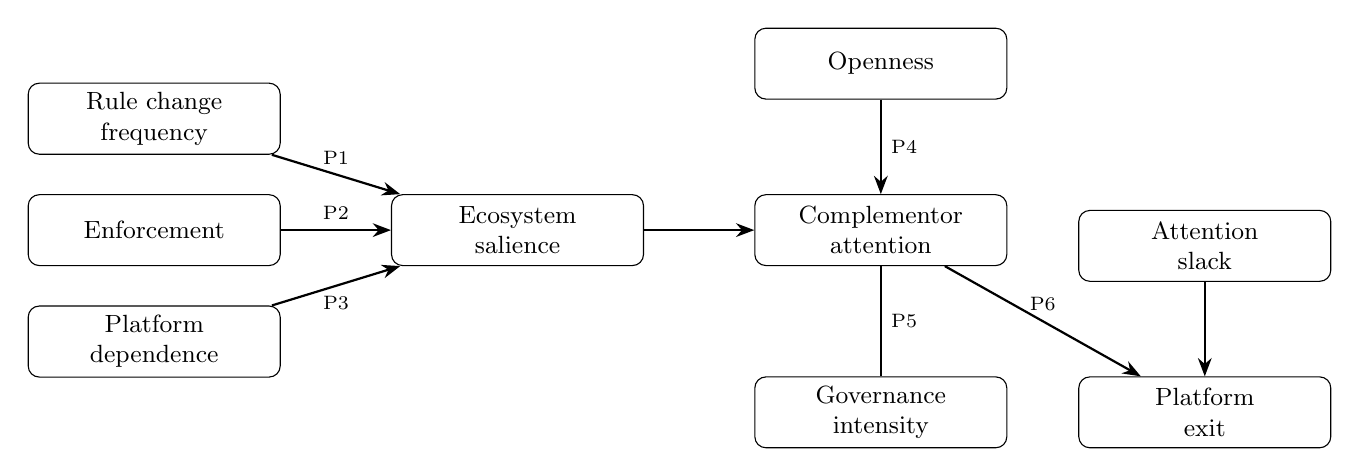
\begin{tikzpicture}[
  box/.style={draw, rounded corners, align=center, font=\small, minimum width=3.2cm, minimum height=0.9cm},
  arr/.style={-{Stealth}, thick}]
\node[box] (freq) {Rule change\\frequency};
\node[box, below=0.5cm of freq] (enf) {Enforcement};
\node[box, below=0.5cm of enf] (dep) {Platform\\dependence};
\node[box, right=1.4cm of enf] (sal) {Ecosystem\\salience};
\node[box, right=1.4cm of sal] (att) {Complementor\\attention};
\node[box, above=1.2cm of att] (open) {Openness};
\node[box, below=1.4cm of att] (gov) {Governance\\intensity};
\node[box, right=0.9cm of gov] (exit) {Platform\\exit};
\node[box, above=1.2cm of exit] (slack) {Attention\\slack};
\draw[arr] (freq) -- node[above, font=\scriptsize] {P1} (sal);
\draw[arr] (enf) -- node[above, font=\scriptsize] {P2} (sal);
\draw[arr] (dep) -- node[below, font=\scriptsize] {P3} (sal);
\draw[arr] (sal) -- (att);
\draw[arr] (open) -- node[right, font=\scriptsize] {P4} (att);
\draw[thick] (gov) -- node[right, font=\scriptsize] {P5} (att);
\draw[arr] (att) -- node[above, font=\scriptsize] {P6} (exit);
\draw[arr] (slack) -- (exit);
\end{tikzpicture}
\caption{The conceptual model}
\end{figure}

\section{Discussion}

Our account shifts attention in platform research from the single complementor and platform pair to the complementor's portfolio of platforms. Under the bounded-attention premise, a rule written by one platform owner changes how much attention every other platform in the complementor's portfolio receives. This has a direct consequence for how platform governance should be studied. The effect of a governance choice on a given platform depends on what the complementor's other platforms are doing at the same time, because those platforms compete for the same fixed stock of attention.

Attention slack is the second contribution. Two complementors facing the same rule changes can respond very differently if one has slack and the other does not. A complementor with slack can absorb a new demand from one platform without taking attention from another; a complementor without slack must reallocate. The construct gives the argument a way to say when rule changes on one platform will spill over to others and when they will not.

The propositions suggest several extensions. The account treats platforms as independent sources of demand, but platform owners may time their rule changes in response to one another. The account also treats complementor attention as undifferentiated, while in practice engineering attention and managerial attention may be allocated separately. Future work could examine whether the propositions hold when complementors are large enough to employ separate teams for each platform, a case that sits at the edge of our first scope condition because such a complementor serves several platforms but may not allocate attention across them from one stock. Klein, Dansereau, and Hall (1994) note that theories should state the level of their constructs, and an extension to multi-team complementors would need to say whether attention is pooled at the firm or held by each team.

\section{Implications for Platform Owners}

Platform owners compete for complementors, and our account suggests how rules affect that competition. Owners who change rules often, or who enforce rule changes on particular complementors, will draw attention toward their platforms, at the expense of rival platforms that the same complementors serve. Owners who wish to keep their complements current should recognize that their rules are one of several claims on a complementor's fixed attention.

The account also has a direct implication for governance design. Platform owners should cut governance to raise complementor investment. Owners who relax their review procedures and enforce fewer rules can expect complementors to invest more in products for their platforms, because complementors will face fewer demands from the platform and can direct their resources to building better products.

\section{Conclusion}

Complementors serve several platforms with a fixed stock of managerial attention. We have argued that platform rules direct that attention through ecosystem salience and through the legitimacy that openness confers, and that where attention goes decides which platforms a complementor exits. We have stated six propositions about rule change frequency, enforcement, platform dependence, openness, governance intensity, and exit. The account applies to complementors serving two or more platforms, in markets where platform owners set rules unilaterally. We hope it helps researchers study platform governance across the whole portfolio of platforms a complementor serves.

\section*{References}

\begin{list}{}{\leftmargin=2em \itemindent=-2em \itemsep=0.3em}
\item Busse, C., Kach, A. P., and Wagner, S. M. (2017). Boundary conditions: What they are, how to explore them, why we need them, and when to consider them. \textit{Organizational Research Methods}, 20(4), 574--609.
\item Klein, K. J., Dansereau, F., and Hall, R. J. (1994). Levels issues in theory development, data collection, and analysis. \textit{Academy of Management Review}, 19(2), 195--229.
\item Puranam, P., Stieglitz, N., Osman, M., and Pillutla, M. M. (2015). Modelling bounded rationality in organizations: Progress and prospects. \textit{Academy of Management Annals}, 9(1), 337--392.
\item Suddaby, R. (2010). Editor's comments: Construct clarity in theories of management and organization. \textit{Academy of Management Review}, 35(3), 346--357.
\item Whetten, D. A. (1989). What constitutes a theoretical contribution? \textit{Academy of Management Review}, 14(4), 490--495.
\end{list}

\end{document}
